\section{Mating Without Corners: Tablebases}\label{sec:tb}

We now bring in the pieces and ask a classical question: without corners, which material can still force
mate? We computed the tablebases of eight pawnless endings, king and one or two pieces against the bare
king, on the ordinary board, on the cylinder and on the torus, where ranks 1 and 8 are joined as well. Chess
on these boards is an old variant~\cite{Pritchard}. Prose sources say that king and rook cannot force mate
on the cylinder, nor king and queen on the torus~\cite{WikiCylinder,HGMCylinder}; we confirm the torus claim,
but the rook mates from 2.80\% of cylinder positions. We found no earlier tablebase for them.

\emph{Rules.} Pieces move as in Section~\ref{sec:rules} and wrap round each glued edge. There is no castling
and no fifty-move rule, and stalemate and bare kings are draws. A position is legal when the kings are not
adjacent, across the seams included, and the side not to move is not in check. Both dimensions of the board
are even, so the coloring of the squares survives the gluing.

\emph{Verification.} Two retrograde solvers, written independently from these rules, agree on every position
of all 24 tables, about 607 million values with either side to move \lab{C2}. On the ordinary board both
reproduce the known longest mates.

\begin{table}[!t]
\centering
\caption{Pawnless Endings Against the Bare King on the Ordinary Board, Cylinder and Torus: Share Won With
White to Move and Longest Mate \lab{C2}}
\label{tab:tb}
\footnotesize
\setlength{\tabcolsep}{4.5pt}
\begin{tabular}{@{}lrrrrrr@{}}
\toprule
& \multicolumn{2}{c}{Ordinary} & \multicolumn{2}{c}{Cylinder} & \multicolumn{2}{c}{Torus} \\
\cmidrule(lr){2-3}\cmidrule(lr){4-5}\cmidrule(l){6-7}
Material & Won (\%) & Mate & Won (\%) & Mate & Won (\%) & Mate \\
\midrule
KQK  & 100    & 10 & 100    & 10 & 0      & --- \\
KRK  & 100    & 16 & 2.80   & 3  & 0      & --- \\
KBBK & 99.98  & 19 & 100    & 14 & 0      & --- \\
KBNK & 99.51  & 33 & 0.0245 & 2  & 0      & --- \\
KNNK & 0.0107 & 1  & 0.0077 & 1  & 0      & --- \\
KRBK & 100    & 16 & 99.74  & 13 & 0.0218 & 1   \\
KRRK & 100    & 7  & 100    & 8  & 100    & 7   \\
KQRK & 100    & 6  & 100    & 5  & 100    & 5   \\
\bottomrule
\end{tabular}

\smallskip
\parbox{\columnwidth}{\footnotesize Mate: longest forced mate in moves; ---: no position is won. KBBK has
the bishops on opposite colors.}
\end{table}

On the cylinder the queen ignores the seam: KQK wins every position, as quickly as on the ordinary board.
KRK, KBNK and KNNK do not, and on the torus not even the queen can force mate
(Table~\ref{tab:tb}).

\emph{KRK and KBNK rarely force mate on the cylinder.} The first and eighth ranks are still edges, but now
closed loops with no corner. The rook wins only 2.80\% of the positions, all from mating nets already
in place, such as Ka3, Rb2 against Ka1: 1.~Rb3 Kh1 2.~Rg3 Ka1 3.~Rg1\#. The rook covers h1 and the
white king h2, the two flight squares across the seam. Bishop and knight win even more rarely: their mate
needs a corner of the bishop's color, and the cylinder has none.

\emph{Bishops on opposite colors win every position on the cylinder}, and faster than on the ordinary board,
although the bishop pair is said not to mate there~\cite{HGMCylinder}.
Here the seam helps the attacker: every diagonal winds round from the first rank to the eighth. The longest
line ends in Ke6, Be1, Bf1 against Ke8: the bishop on f1 checks along f1--h3--a4--e8, across the seam, and
the bishop on e1 covers d8 and f8.

\emph{On the torus, of the eight endings, only KRRK and KQRK force mate}, and they win from every position. KRBK wins only where
a mate in one is already set up, and the bishop pair has mating positions that no legal white move can
produce.

\emph{Twisted boards.} KRK wins everywhere on the M\"obius strip (files a and h joined, ranks reversed), but
only $0.66\%$ on the Klein bottle, which also joins ranks 1 and 8 \lab{C2}.

\subsection{King and Pawn Against King}\label{sec:kpk}

We solved every legal KPK position on the $8\times8$ ordinary board and cylinder twice, with our
king-and-pawn solver of Section~\ref{sec:kings} (all four promotions) and with a separately written KPK
solver (queen promotion only). They agree on all 326,640 cylinder positions and differ on exactly 6
ordinary-board positions, where only a rook promotion wins, such as Ka4, Pb7 against
Ka6 \lab{C2}. Table~\ref{tab:kpk} gives the counts; the cylinder has fewer legal positions, since the kings
may not touch across the seam and, with white to move, the black king may not stand where the white
pawn attacks across the seam.

\begin{table}[!t]
\centering
\caption{King and Pawn Against King: Legal Positions and White Wins on the $8\times8$ Ordinary Board and
Cylinder \lab{C2}}
\label{tab:kpk}
\footnotesize
\begin{tabular}{@{}lrrrr@{}}
\toprule
& \multicolumn{2}{c}{White to move} & \multicolumn{2}{c}{Black to move} \\
\cmidrule(lr){2-3}\cmidrule(l){4-5}
Board & Legal & White wins & Legal & White wins \\
\midrule
Ordinary & 163,328 & 124,960 & 168,024 & 97,604 \\
Cylinder & 160,656 & 126,736 & 165,984 & 92,760 \\
\bottomrule
\end{tabular}
\end{table}

\begin{figure}[!t]
\centering
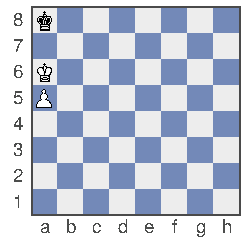
\includegraphics[width=0.26\columnwidth]{figures/kpk_rookpawn.pdf}
\caption{Ka6, Pa5 against Ka8, with either side to move: a white win on the cylinder (files a and h adjacent),
a draw on the ordinary board.}
\label{fig:kpk_rookpawn}
\end{figure}

Fig.~\ref{fig:kpk_rookpawn} shows the classic rook-pawn draw: on the ordinary board the black king cannot be
driven out of the corner without stalemate. On the cylinder we may shift every man four files to the right,
which gives Ke6, Pe5 against Ke8, the textbook win whoever is to move. Back on the a-file, with black to move,
play goes 1\ldots~Kb8 2.~Kh7 Kb7 3.~a6+, and the pawn promotes under the king, which guards a7 and a8 from h7.

Of the positions legal on both boards, 16,538 ordinary-board draws become cylinder wins. The seam also
helps the defender, since a king on the h-file now stands beside an a-pawn: 15,930 ordinary-board wins
become cylinder draws. Zugzwang, the engine of the tr\'ebuchet, is more common on the cylinder: 216
reciprocal zugzwangs (white to move draws, black to move loses) against 160 on the ordinary board
\lab{C2}.

\begin{table}[!t]
\centering
\caption{King and Pawn Against King on $\cyl{n}$: White-to-Move Wins and Reciprocal Zugzwangs \lab{C2}}
\label{tab:oddw}
\footnotesize
\begin{tabular}{@{}lrrr@{}}
\toprule
$n$ & Legal, white to move & White wins (\%) & Reciprocal zugzwangs \\
\midrule
3 & 5,706   & 53.00 & 0   \\
4 & 16,008  & 65.87 & 208 \\
5 & 34,350  & 73.92 & 95  \\
6 & 63,036  & 76.55 & 132 \\
7 & 104,370 & 77.49 & 175 \\
8 & 160,656 & 78.89 & 216 \\
\bottomrule
\end{tabular}
\end{table}

\emph{Other widths.} Table~\ref{tab:oddw} covers $\cyl{n}$ for $n=3,\dots,8$, where two independently
written solvers agree \lab{C2}; one widened solver gives 79.41\% and 79.94\% for $n=9,10$ \lab{C1}. Odd
and even widths behave alike: the win rate rises with $n$, and from $n=4$ on the share of reciprocal zugzwangs falls,
from 1.30\% to 0.13\% at $n=8$. The tr\'ebuchet of Fig.~\ref{fig:trebuchet_2025} is a mutual zugzwang (the side to
move loses either way) for $4\le n\le8$ \lab{C2} and $n=9$ \lab{C1}, and illegal on $\cyl{3}$. Ka3, Pa2 against
Ka5, a draw on the ordinary board, is a reciprocal zugzwang for $4\le n\le8$ \lab{C2} and $n=9,10$ \lab{C1}. On $\cyl{3}$, Ka1, Pa7 against Ka3
wins at once: a8=Q checks along the a-file, which covers a4, and the wrapped diagonals and the white king cover
the other flight squares \lab{C2}.

\emph{A pawn each.} With all promotions but at most one new piece, our solver decides 89\% of the 14.6 million
KPKP placements on the cylinder (14.9 million on the ordinary board) and 83\% on the ordinary board \lab{C1}
(placements with an e.p.\ right pending are not enumerated). Of the positions decided on both,
10\% change result, three quarters of them to a draw, and 576 pairs of reciprocal zugzwangs exist only on the
cylinder, 20 of them mutual: in Ka3, Ph2 against Kg2, Ph3 whoever moves loses, since Ka3 reaches the
locked pawns across the seam; a second solver agrees on a sample \lab{C2}.
